\documentclass[12pt,a4paper,final]{article}
\usepackage[left=2.5cm,right=2.5cm,top=2.5cm,bottom=2.5cm]{geometry}

%% IDIOMA
\usepackage[utf8]{inputenc}
\usepackage[portuguese]{babel}

%% TRANSFORMAÇÕES ESTILO CSS
\usepackage{graphicx}

%% ESTÉTICA
\usepackage{enumerate}
\usepackage{booktabs}
\usepackage{amsmath, amsthm, amssymb, amsfonts}
\usepackage{multirow}
\usepackage[hyphens]{url}
\usepackage{subfig}

%% FONTE
\usepackage[T1]{fontenc}
%\usepackage[sc]{mathpazo} % Palatino with smallcaps
\usepackage{mathptmx}
\usepackage{eulervm} % Euler math

%% TIPOGRAFIA
\usepackage{parskip}
\usepackage[activate={true,nocompatibility},final,tracking=true,kerning=true,spacing=true,factor=1100,stretch=10,shrink=10]{microtype}

%% CODIGO
\usepackage{listings}
\usepackage{color}

\definecolor{dkgreen}{rgb}{0,0.6,0}
\definecolor{gray}{rgb}{0.5,0.5,0.5}
\definecolor{mauve}{rgb}{0.58,0,0.82}

\lstset{frame=tb,
  aboveskip=3mm,
  belowskip=3mm,
  showstringspaces=false,
  columns=flexible,
  basicstyle={\small\ttfamily},
  numbers=none,
  numberstyle=\tiny\color{gray},
  keywordstyle=\color{blue},
  commentstyle=\color{dkgreen},
  stringstyle=\color{mauve},
  breaklines=true,
  breakatwhitespace=true,
  tabsize=3
}

\title{Relatório 10 de TCC2/IC}
\author{Ly Sandro Amorim de Campos Salles\\Departamento de Física\\Universidade Federal do Paraná}
\date{\today}

\begin{document}
	\maketitle

  Desde o último encontro foram realizadas as seguintes atividades:

  Obtenção de cinco conjuntos de 20000 pontos, para uma simulação que utilizou a vizinhança de Moore (8 células adjacentes), e considerou $L=50$ e $q\in\{$ 
  $0.1,$ $0.2,$ $0.3,$ $0.4,$ $0.5,$ $0.6,$ $0.7,$ $0.8,$ $0.9,$
  $1,$ $1.2,$ $1.4,$ $1.6,$ $1.8,$ 
  $2,$ $2.2,$ $2.4,$ $2.6,$ $2.8,$ 
  $3,$ $3.2,$ $3.4,$ $3.6,$ $3.8,$
  $4,$ $4.2,$ $4.4,$ $4.6,$ $4.8,$
  $5,$ $5.2,$ $5.4,$ $5.6,$ $5.8,$
  $6,$ $6.2,$ $6.4,$ $6.6,$ $6.8,$
  $7,$ $7.2,$ $7.4,$ $7.6,$ $7.8,$
  $8,$ $8.2,$ $8.4,$ $8.6,$ $8.8,$
  $9,$ $9.2,$ $9.4,$ $9.6,$ $9.8,$ $10,$
  $11,$ $12,$ $13,$ $14,$ $15,$ $16,$ $17,$ $18,$ $19,$ $20,$
  $22,$ $24,$ $26,$ $28,$ $30,$ $32,$ $34,$ $36,$ $38,$ $40,$
  $42,$ $44,$ $46,$ $48,$ $50,$ $52,$ $54,$ $56,$ $58,$ $60,$
  $65,$ $70,$ $75,$ $80,$ $85,$ $90,$ $95,$ $100,$ $110,$
  $120,$ $130,$ $140,$ $150,$ $160,$ $170,$ $180,$ $190,$
  $200,$ $220,$ $240,$ $260,$ $280,$ $300,$ $320,$ $340,$ $360,$ $380,$
  $400,$ $420,$ $440,$ $460,$ $480,$ $500,$ $520,$ $540,$ $560,$ $580,$
  $600,$ $620,$ $640,$ $660,$ $680,$ $700,$ $720,$ $740,$ $760,$ $780,$
  $800,$ $820,$ $840,$ $860,$ $880,$ $900,$ $920,$ $940,$ $960,$ $980,$
  $1000\}$. 

  Obtenção de cinco conjuntos de 10000 pontos, para uma simulação que utilizou a vizinhança de Moore (8 células adjacentes), e considerou $L\in\{$ $100,$ $250,$ $500$ $\}$  e $q\in\{$ 
  $0.2,$ $0.4,$ $0.6,$ $0.8,$
  $1,$ $1.2,$ $1.4,$ $1.6,$ $1.8,$ 
  $2,$ $2.2,$ $2.4,$ $2.6,$ $2.8,$ 
  $3,$ $3.2,$ $3.4,$ $3.6,$ $3.8,$
  $4,$ $4.2,$ $4.4,$ $4.6,$ $4.8,$
  $5,$ $5.2,$ $5.4,$ $5.6,$ $5.8,$
  $6,$ $6.2,$ $6.4,$ $6.6,$ $6.8,$
  $7,$ $7.2,$ $7.4,$ $7.6,$ $7.8,$
  $8,$ $8.2,$ $8.4,$ $8.6,$ $8.8,$
  $9,$ $9.2,$ $9.4,$ $9.6,$ $9.8,$ $10,$
  $11,$ $12,$ $13,$ $14,$ $15,$ $16,$ $17,$ $18,$ $19,$ $20,$
  $22,$ $24,$ $26,$ $28,$ $30,$ $32,$ $34,$ $36,$ $38,$ $40,$
  $42,$ $44,$ $46,$ $48,$ $50$ $\}$. 

  Obtenção de cinco conjuntos de 10000 pontos, para uma simulação que utilizou a vizinhança de Moore (8 células adjacentes), e considerou $L=500$  e $q\in\{$ 
  $0.2,$ $0.4,$ $0.6,$ $0.8,$
  $1,$ $1.2,$ $1.4,$ $1.6,$ $1.8,$ 
  $2,$ $2.2,$ $2.4,$ $2.6,$ $2.8,$ 
  $3,$ $3.2,$ $3.4,$ $3.6,$ $3.8,$
  $4,$ $4.2,$ $4.4,$ $4.6,$ $4.8,$
  $5,$ $5.2,$ $5.4,$ $5.6,$ $5.8,$
  $6,$ $6.2,$ $6.4,$ $6.6,$ $6.8,$
  $7,$ $7.2,$ $7.4,$ $7.6,$ $7.8,$
  $8,$ $8.2,$ $8.4,$ $8.6,$ $8.8,$
  $9,$ $9.2,$ $9.4,$ $9.6,$ $9.8,$ $10$ $\}$. 

  Cálculo das afinidades para o conjunto de dados com $L=500$ e vizinhança de Von Neumann. 
  
  Cálculo das afinidades para os conjuntos de dados com $L\in\{50, 100, 250, 500\}$.

  As Figuras \ref{fig:VonNeumannAfinidades}, \ref{fig:VonNeumannDerivadaAfinidade} e \ref{fig:VonNeumannMaximosDerivada} resumem todas as informações que foram encontradas sobre o comportamento da afinidade quando considerada a vizinhança de Von Neumann (células ortogonais) e $L\in\{50, 100, 250, 500\}$.

  \begin{figure}[h]
    \centering
    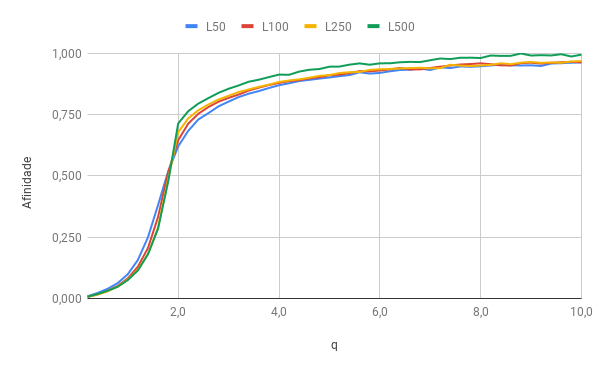
\includegraphics[width=.7\linewidth]{VonNeumannAfinidades.png}
    \caption{Gráficos das afinidades para $L\in\{50, 100, 250, 500\}$ considerando a vizinhança de Von Neumann. Percebe-se que menores valores de $L$ geram curvas mais suaves em relação a valores maiores de $L$.}
    \label{fig:VonNeumannAfinidades}
  \end{figure}

  \begin{figure}[h]
    \centering
    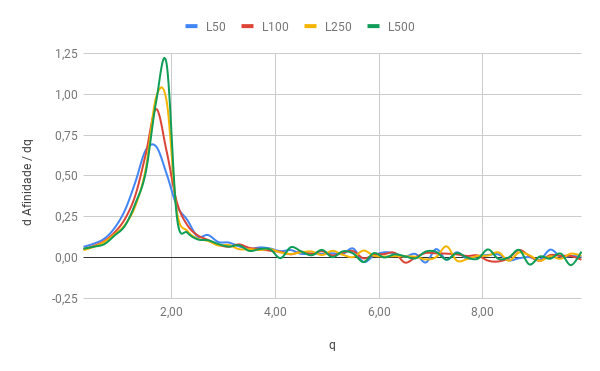
\includegraphics[width=.7\linewidth]{VonNeumannDerivadaAfinidade.png}
    \caption{Derivada da afinidade em relação a $q$ para $L\in\{50, 100, 250, 500\}$ e vizinhança de Von Neumann. Os máximos representam a velocidade de crescimento da afinidade no ponto crítico.}
    \label{fig:VonNeumannDerivadaAfinidade}
  \end{figure}

  \begin{figure}[h]
    \centering
    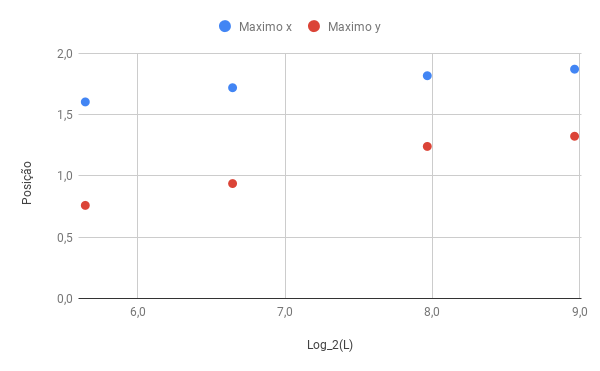
\includegraphics[width=.7\linewidth]{VonNeumannMaximosDerivada.png}
    \caption{Posições x e y para os máximos da derivada da afinidade com Vizinhança de Von Neumann. O eixo x foi tomado como $\mathrm{log_2}(L)$ pois os dados têm uma dependência aproximadamente linear quando considerado isso. A coordenada x do máximo é dada por $M_{x}(L) = \mathrm{MAX}(d Afinidade / dq) \approx 0.080\cdot\mathrm{log_2}(L)+1.172$. A coordenada y do máximo é dada por $M_{x}(L) = \mathrm{MAX}(d Afinidade / dq) \approx 0.178\cdot\mathrm{log_2}(L)-0.234$.}
    \label{fig:VonNeumannMaximosDerivada}
  \end{figure}

  As Figuras \ref{fig:MooreAfinidades}, \ref{fig:MooreDerivadaAfinidade} e \ref{fig:MooreMaximosDerivada} resumem todas as informações que foram encontradas sobre o comportamento da afinidade quando considerada a vizinhança de Moore (células ortogonais e diagonais) e $L\in\{50, 100, 250, 500\}$.

  \begin{figure}[h]
    \centering
    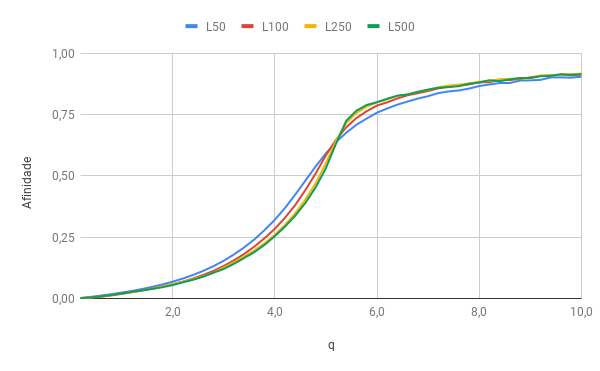
\includegraphics[width=.7\linewidth]{MooreAfinidades.png}
    \caption{Gráficos das afinidades para $L\in\{50, 100, 250, 500\}$ considerando a vizinhança de Moore. Percebe-se, novamente, que menores valores de $L$ geram curvas mais suaves em relação a valores maiores de $L$.}
    \label{fig:MooreAfinidades}
  \end{figure}

  \begin{figure}[h]
    \centering
    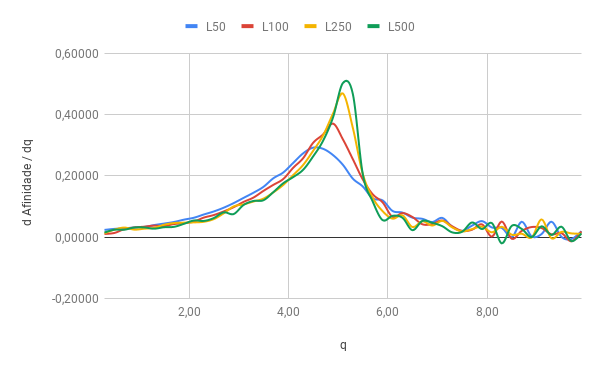
\includegraphics[width=.7\linewidth]{MooreDerivadaAfinidade.png}
    \caption{Derivada da afinidade em relação a $q$ para $L\in\{50, 100, 250, 500\}$ e vizinhança de Moore. Os máximos representam a velocidade de crescimento da afinidade no ponto crítico.}
    \label{fig:MooreDerivadaAfinidade}
  \end{figure}

  \begin{figure}[h]
    \centering
    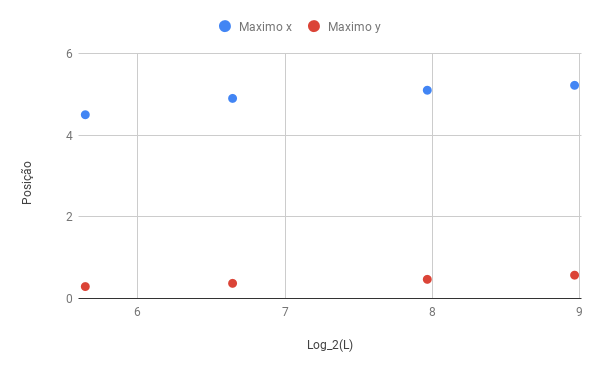
\includegraphics[width=.7\linewidth]{MooreMaximosDerivada.png}
    \caption{Posições x e y para os máximos da derivada da afinidade com Vizinhança de Moore. O eixo x foi tomado como $\mathrm{log_2}(L)$ pois os dados têm uma dependência aproximadamente linear quando considerado isso. A coordenada x do máximo é dada por $M_{x}(L) = \mathrm{MAX}(d Afinidade / dq) \approx 0.208\cdot\mathrm{log_2}(L)+3.412$. A coordenada y do máximo é dada por $M_{x}(L) = \mathrm{MAX}(d Afinidade / dq) \approx 0.083\cdot\mathrm{log_2}(L)-0.178$.}
    \label{fig:MooreMaximosDerivada}
  \end{figure}

  Foi desenvolvido o seguinte de resumo para apresentação ao EVINCI:\\
  \textit{Utilizando um autômato celular bidimensional desenvolvido por Dietrich Stauffer e Gérard Weisbuch para simulações de compra e venda de agentes em um mercado, determinamos a intensidade com que esses agentes tendem a tomar decisões em conjunto, denominada afinidade. Isso foi feito considerando vizinhanças de Moore e Von Neumann. Desenvolvemos duas interpretações para a variável que determina a velocidade do sistema: liquidez de mercado, e volatilidade. Essas simulações foram feitas para números diferentes de agentes, variando de 2500 a 250000. Descobrimos, nessa análise positiva, que a afinidade é uma função sigmóide da liquidez do mercado, variando com o número de agentes nesse mercado. Com base nesses dados percebemos que, para mercados com alta liquidez, como o de alimentos, a tendência a aglomeração de agentes é alta, o que explica as Centrais de Abastecimento CEASA. Analogamente, quando a liquidez do mercado é baixa, como no caso dos itens de colecionador e figurinhas de copa do mundo, a tendência de aglomeração é menor, fazendo com que existam mais aglomerados esparsamente distribuídos, como grupos de troca de figurinhas em várias praças de uma mesma cidade. Com a análise de volatilidade foi percebido um comportamento semelhante ao de mercados financeiros. Aproveitando a forma com que computadores geram números aleatórios também foi possível verificar se os autômatos celulares estudados apresentavam comportamento caótico. Colateralmente foi desenvolvido um algoritmo de contagem de aglomerados para autômatos celulares em duas dimensões que se mostrou mais eficiente do que os utilizados atualmente.}\\ \textbf{Palavras-chave:} microeconomia, autômato celular, aglomeração, análise positiva, liquidez de mercado, volatilidade de mercado, estocasticidade, modelagem, econofísica.

  Para os próximos dias, estas serão as tarefas realizadas:
  \begin{enumerate}
    \item Verificação de comportamento caótico para o autômato celular considerando as vizinhanças de Moore e Von Neumann;
    \item Demonstração matemática do Algoritmo de Contagem de Aglomerados utilizado;
    \item Desenvolvimento da explicação que considera $q$ como liquidez;
    \item Desenvolvimento da explicação que considera $q$ como volatilidade;
    \item Explicação do porquê de o limiar intrínseco a cada célula ser considerado como um determinador do momento certo para vender ou comprar, no caso de $q$ ser considerado como liquidez;
    \item Leitura de Referênciais Teóricos apropriados para os trabalhos desenvolvidos;
    \item Escrita do TCC.
	\end{enumerate}

\end{document}
